\documentclass[12pt]{scrartcl}

\usepackage{amsthm}
\usepackage{ocgx}
\usepackage{amsmath}
\usepackage{graphicx}

\title{Lecture Notes week 1}
\author{\"Omer \c Sakar}
\date{\today}

\newtheorem{defi}{Definition}
\newtheorem{theo}{Theorem}

\usepackage{tikz}
\usetikzlibrary{shapes,backgrounds}


\begin{document}
\maketitle
\tableofcontents
\newpage

\section{Lecture 1}

\subsection{Bayes' Rule}
Given events $A$ and $B$:\newline

\begin{defi}
 	The Conditional Probability $P(A | B) = \frac{P(A \cap B) }{P(B)},\ 	 with\ P(B)\ >\ 0.$
\end{defi}

\begin{figure}[h]
	\centering
	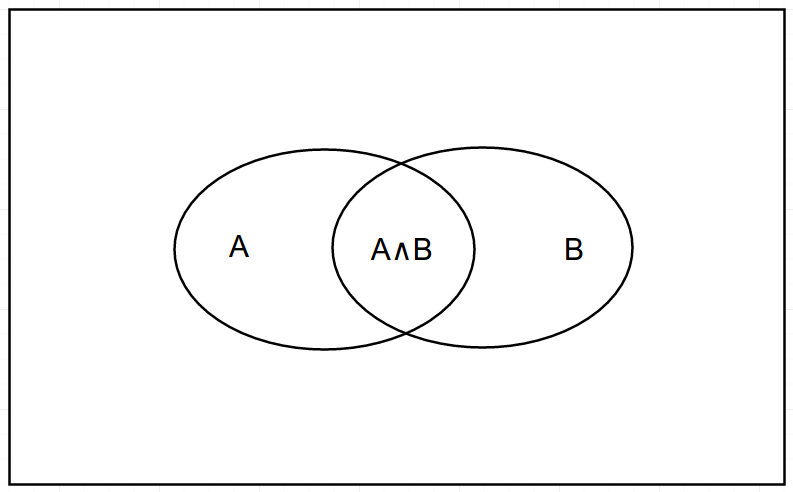
\includegraphics[width=0.3\textwidth]{./images/venn_diagram.png}
	\captionof{figure}{Visual representation of Bayes' Rule}    
    \label{fig:formal_proof_ties}
\end{figure}

Example: There are 40 Math students of which 15 are girls and there are 50 Computer Science students of which 10 are girls.\newline
Let $A\ =\ randomly\ chosen\ student\ is\ a\ girl$ and $B\ =\ randomly\ chosen\ student\ is\ a\ math\ student$.
\newline

$P(A | B) = \frac{P(A \cap B)}{P(B)} = \frac{\ \ \frac{15}{90}\ \ }{\frac{40}{90}} = \frac{3}{8}$\newline

\noindent And from Bayes' Rule follows $\Rightarrow P(A \cap B) = P(A | B)\cdot P(B) = P(B|A)\cdot P(A), P(A) > 0$.

Thus we can rewrite it as:
\begin{defi}
 	The Conditional Probability $P(B | A) = \frac{P(A | B)\cdot P(B) }{P(A)}.$
\end{defi}

\subsubsection{Full Probability Formula}
\begin{defi}
	$P(A) = P(B) \cdot P(A | B) + P(\bar{B})\cdot P(A | \bar{B})$
\end{defi}
\noindent Example: $P(B | A) = \frac{P(A | B)\cdot P(B)}{P(A)} = \frac{\ \frac{40}{90}\cdot \frac{3}{8}\ }{\frac{25}{90}} = \frac{3}{8}$\newline

\subsection{A Herding Experiment}
Envelope 1 contains 8 red and 4 blue domino pieces (R) and envelope 1 contains 4 red and 8 blue domino pieces (B).\newline
$P(R) = P(B) = \frac{1}{2} $\newline
The first person that draws either a red or blue piece.\newline
$P(R | (saw) blue) = \frac{P(blue | R)\cdot P(R)}{P(blue)}$.

\noindent$P(blue) = P(R)\cdot P(blue |R) + P(B)\cdot P(blue | B) = \frac{1}{2}\cdot \frac{4}{12} + \frac{1}{2}\cdot \frac{8}{12} = \frac{1}{2}$

\noindent$P(R | blue) = \frac{\frac{4}{12}\cdot \frac{1}{2}}{\frac{1}{2}} = \frac{1}{3} < \frac{1}{2}\
 and\ P(B | blue) = \frac{\frac{8}{12}\cdot \frac{1}{2}}{\frac{1}{2}} = \frac{2}{3} > \frac{1}{2}$



\noindent Now lets look at when a second person draws.
\begin{defi}
	$D_{i} = \{blue\}\ or\ \{red\}\ -\ what\ person\ i\ says\ they\ saw$
\end{defi}
\begin{defi}
$E_{i} = \{blue\}\ or\ \{red\}\ -\ what\ person\ i\ saw$
\end{defi}
\noindent Lets say that the first person says what he sees ($D_{1} = E_{1}$)

\noindent$P(B | blue, blue) = \frac{P(B)\cdot P(blue, blue | B)}{P(blue, blue)}$

\noindent$P(blue, blue) = \frac{1}{2}\cdot (\frac{2}{3})^{2} + \frac{1}{2}\cdot (\frac{2}{3})^{2} = \frac{5}{18}$

\noindent Thus $P(B | blue, blue) = \frac{\frac{1}{2}\cdot (\frac{2}{3})^{2}}{\frac{5}{18}} = \frac{4}{5} > \frac{1}{2}$

\noindent Conclusion: If $D_{1} = \{blue\}$ and $E_{2} = \{blue\} \implies D_{2} = \{blue \}$

\newpage
\section{Lecture 2} 


\end{document}




